\documentclass[border=5mm]{standalone}
\usepackage{tikz}
\usetikzlibrary{calc, intersections}

\begin{document}
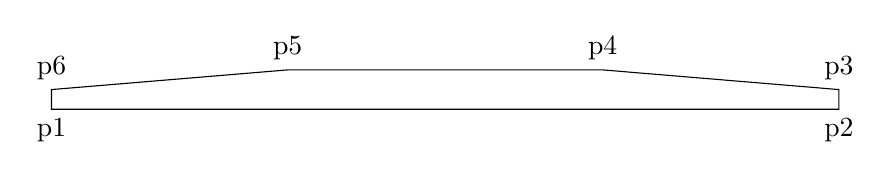
\begin{tikzpicture}

\coordinate [label=below:p1] (m1) at (0,0);
\coordinate [label=below:p2] (m2) at (10,0);
\coordinate [label=above:p3] (m3) at (10,0.25);
\coordinate [label=above:p4] (m4) at (7,0.5);
\coordinate [label=above:p5] (m5) at (3,0.5);
\coordinate [label=above:p6] (m6) at (0,0.25);

\draw (m1) -- (m2) -- (m3) -- (m4) -- (m5) -- (m6) --cycle;

\end{tikzpicture}
\end{document}

